% \documentclass[t]{beamer}
\documentclass{beamer}
\usepackage{minted}
\usepackage{tikz}
\usepackage{amsmath}
\usepackage{adjustbox}
\usepackage{turnstile}
%\usetheme{Boadilla}

\setminted{fontsize=\footnotesize}


\title{Synchronous single initiator spanning tree algorithm using flooding}
\author{Siddharth Bhat, Anurag Chaturvedi, Hitesh Kaushik}
\date{\today}

\begin{document}
\begin{frame}
\titlepage
\end{frame}

\begin{frame}
    \frametitle{Introduction}
    \begin{itemize}
        \item We use BFS to compute a spanning tree of a graph. \pause
        \item We can distribute the sequential algorithm assuming \textit{synchronous communication}. \pause
        \item \textbf{Refresher:} Algorithm proceeds in rounds. All messages sent at round $i$ are received at round $i$. \pause
        \item \textbf{Flood:} everyone sends a message to their neighbours. Think flood fill.
            
\includegraphics[width=0.05\paperwidth]{flood-fill.png}
    \end{itemize}
\end{frame}


% algorithm explanation
\begin{frame}
    \frametitle{Example}
    \begin{figure}
    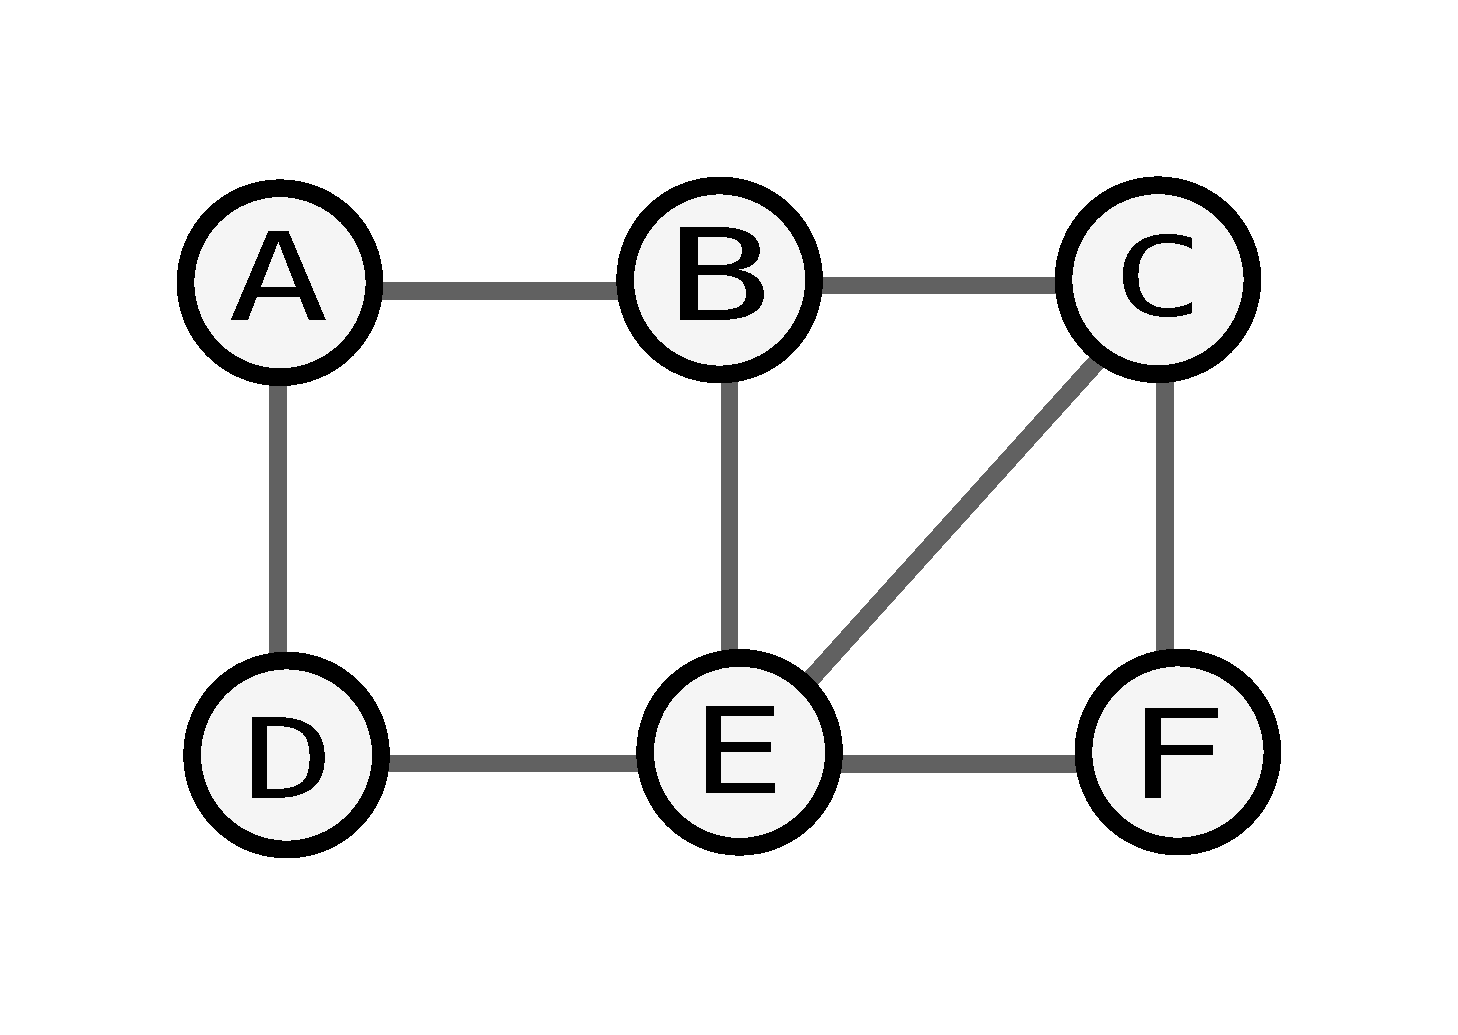
\includegraphics[width=0.5\paperwidth]{base.pdf}
    \end{figure}
\end{frame}

\begin{frame}
    \frametitle{Example}
    \begin{figure}
    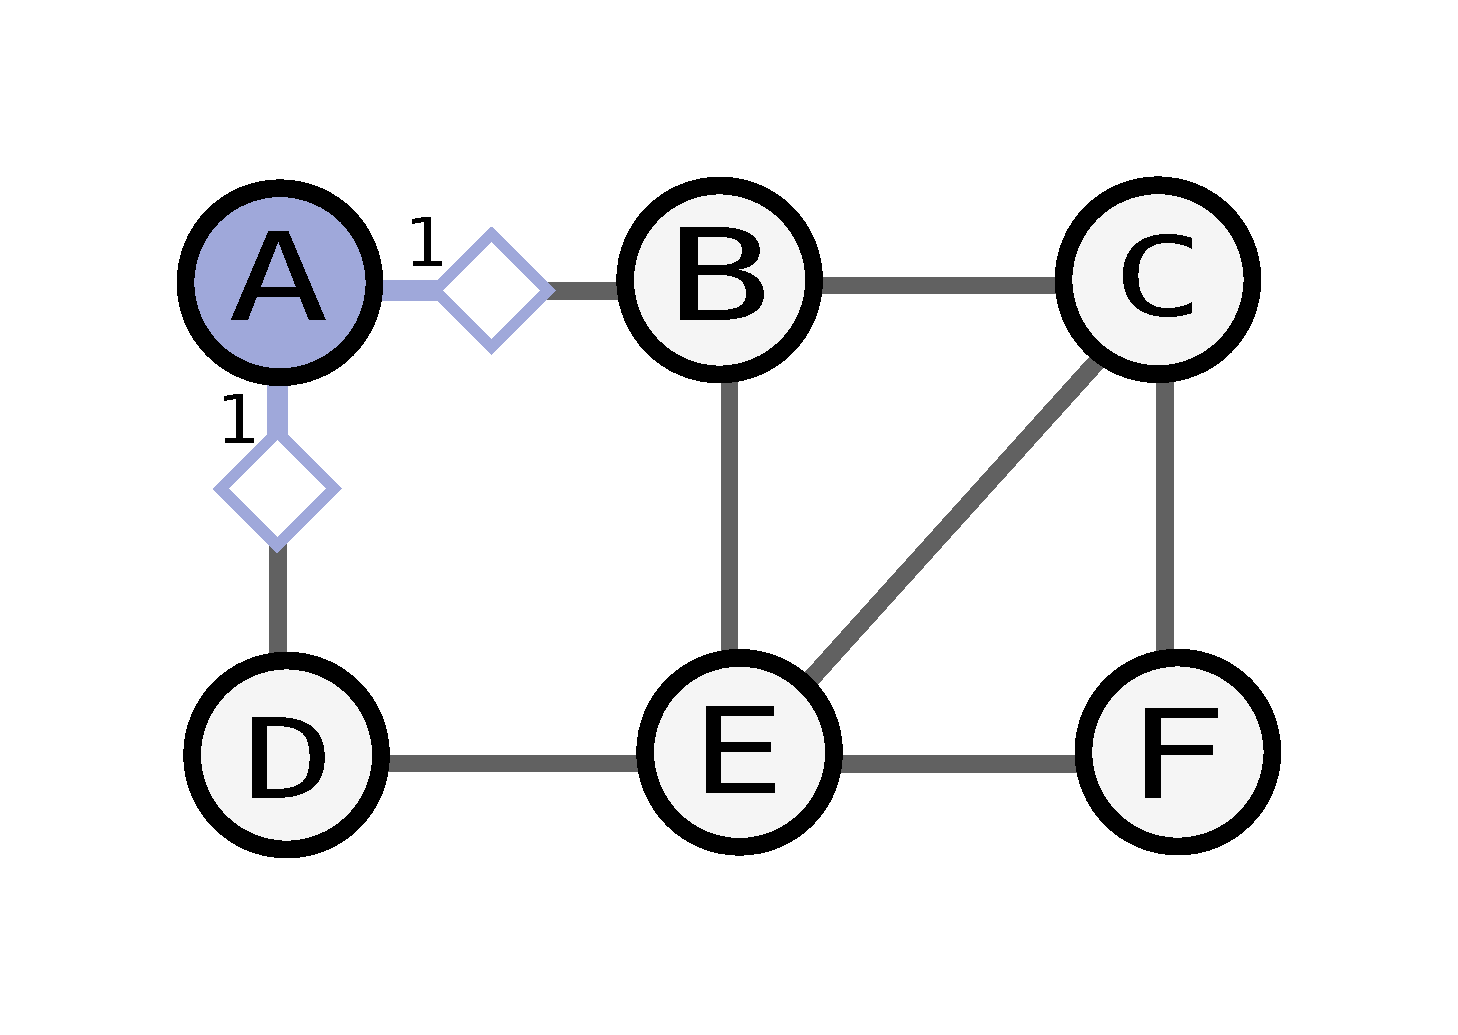
\includegraphics[width=0.5\paperwidth]{round1.pdf}
    \end{figure}
\end{frame}

\begin{frame}
    \frametitle{Example}
    \begin{figure}
    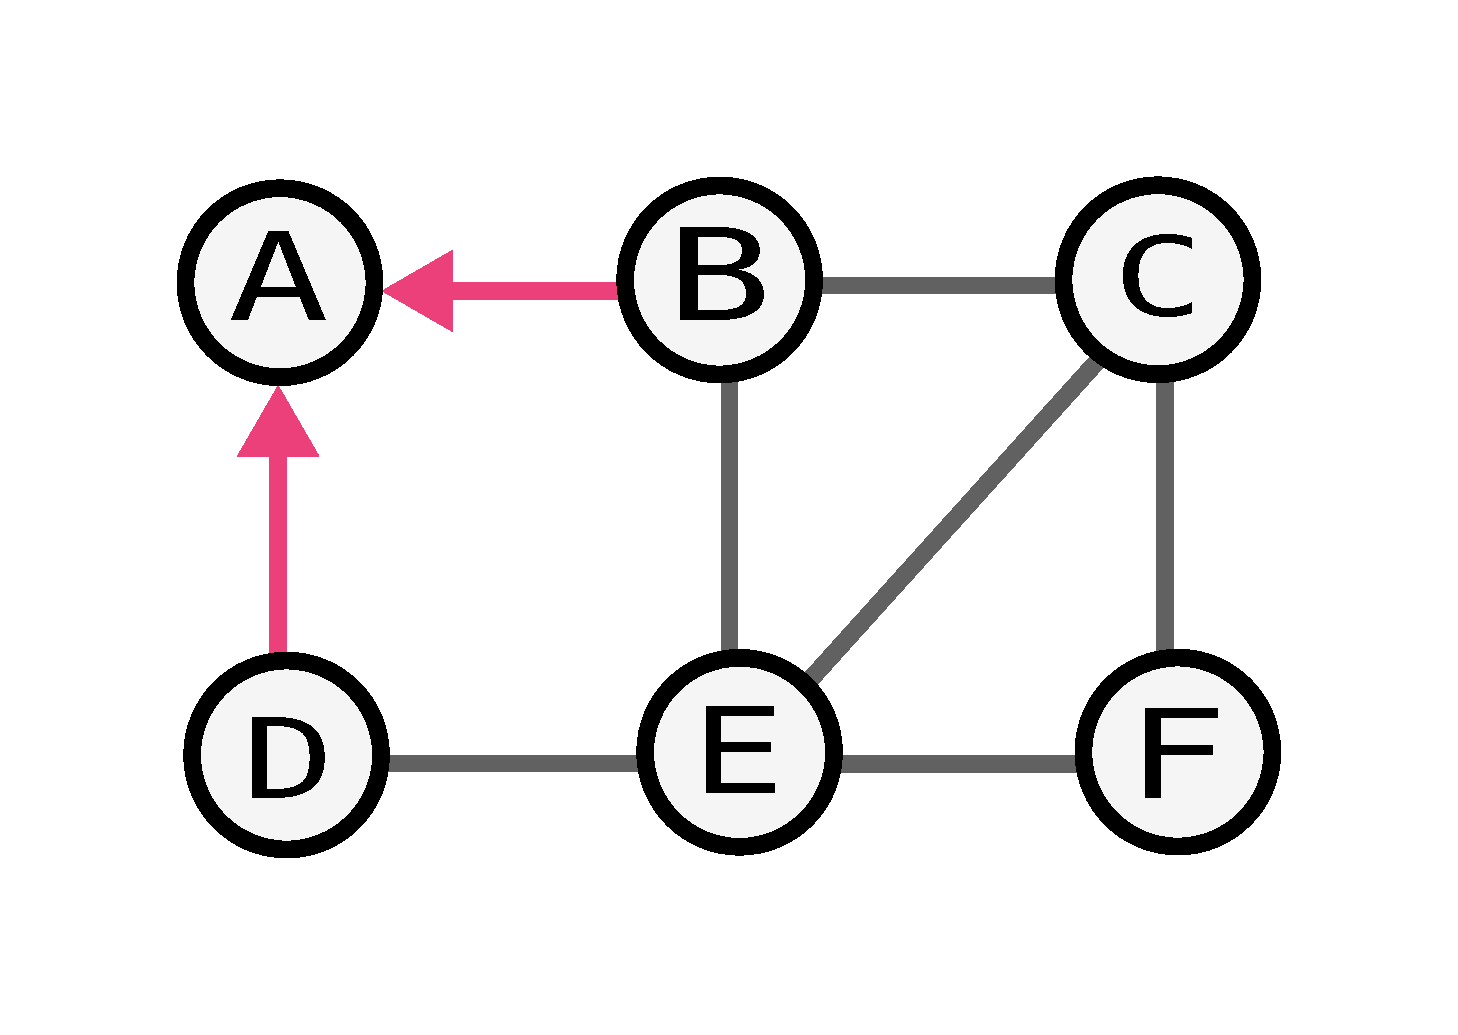
\includegraphics[width=0.5\paperwidth]{round1-end.pdf}
    \end{figure}
\end{frame}


\begin{frame}
    \frametitle{Example}
    \begin{figure}
    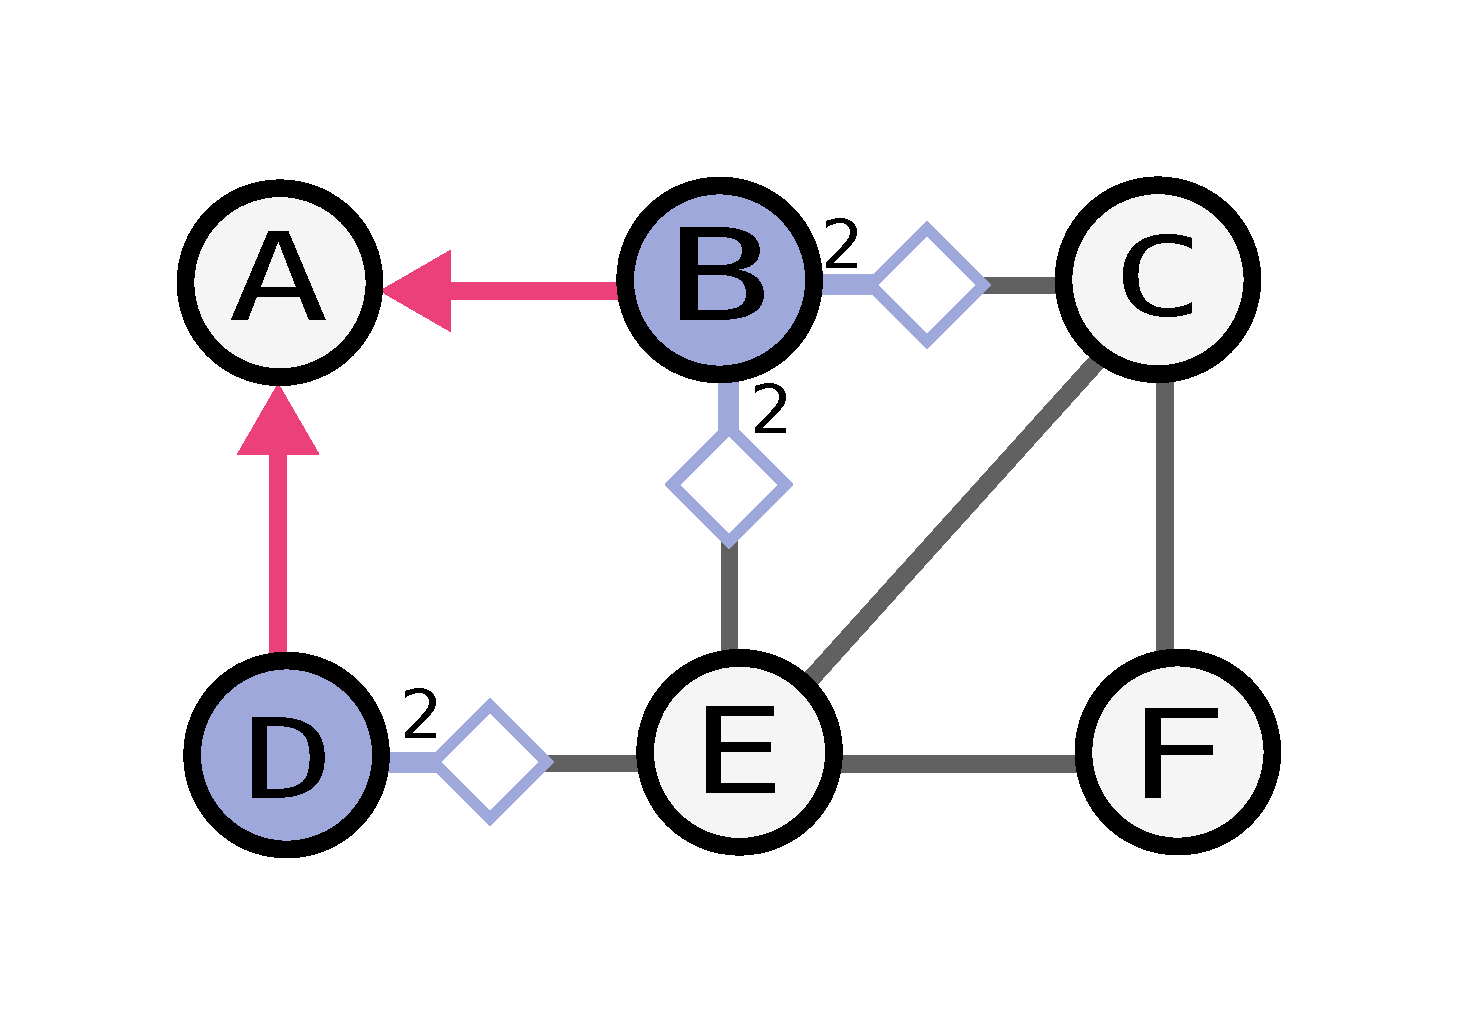
\includegraphics[width=0.5\paperwidth]{round2.pdf}
    \end{figure}
\end{frame}


\begin{frame}
    \frametitle{Example}
    \begin{figure}
    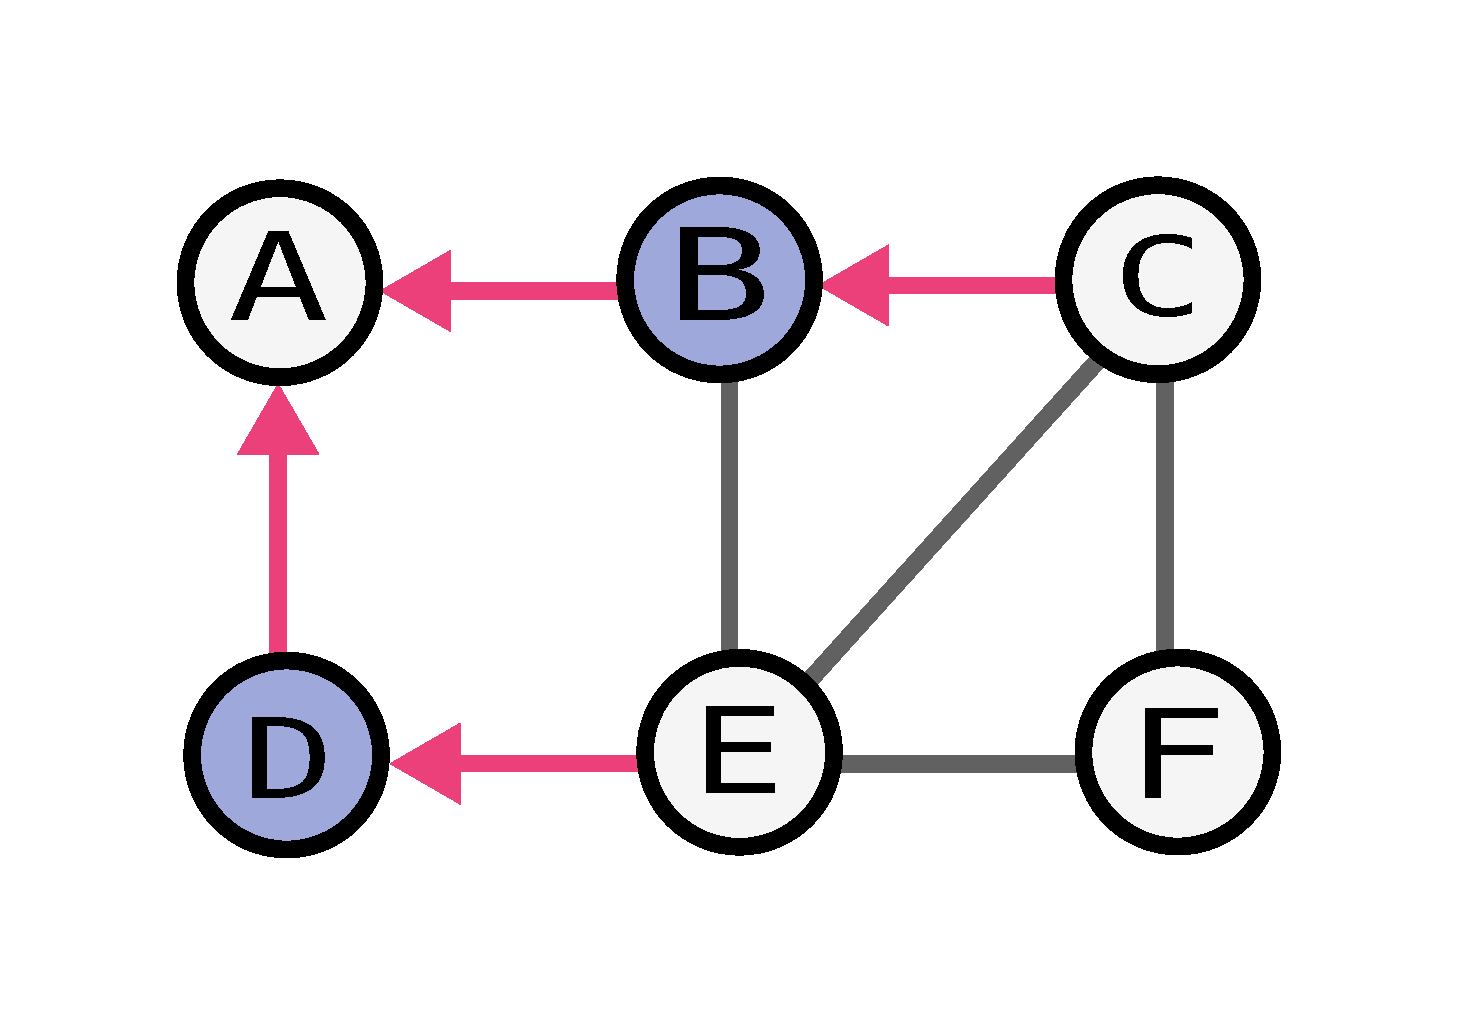
\includegraphics[width=0.5\paperwidth]{round2-end.pdf}
    \end{figure}
\end{frame}


\begin{frame}
    \frametitle{Example}
    \begin{figure}
    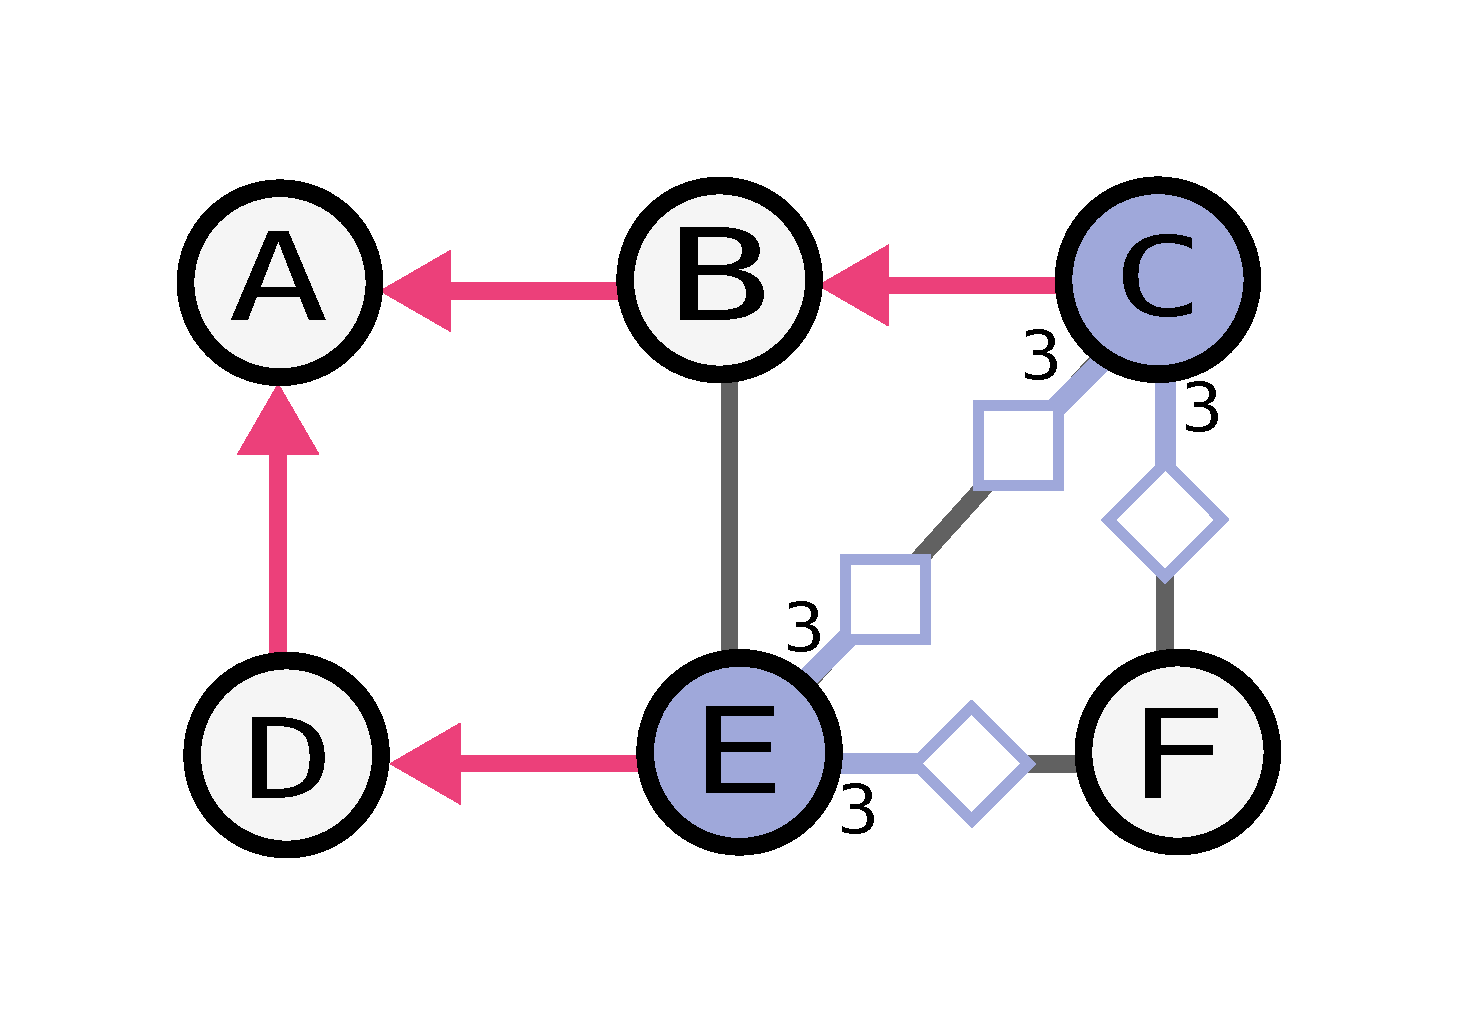
\includegraphics[width=0.5\paperwidth]{round3.pdf}
    \end{figure}
\end{frame}


\begin{frame}
    \frametitle{Example}
    \begin{figure}
    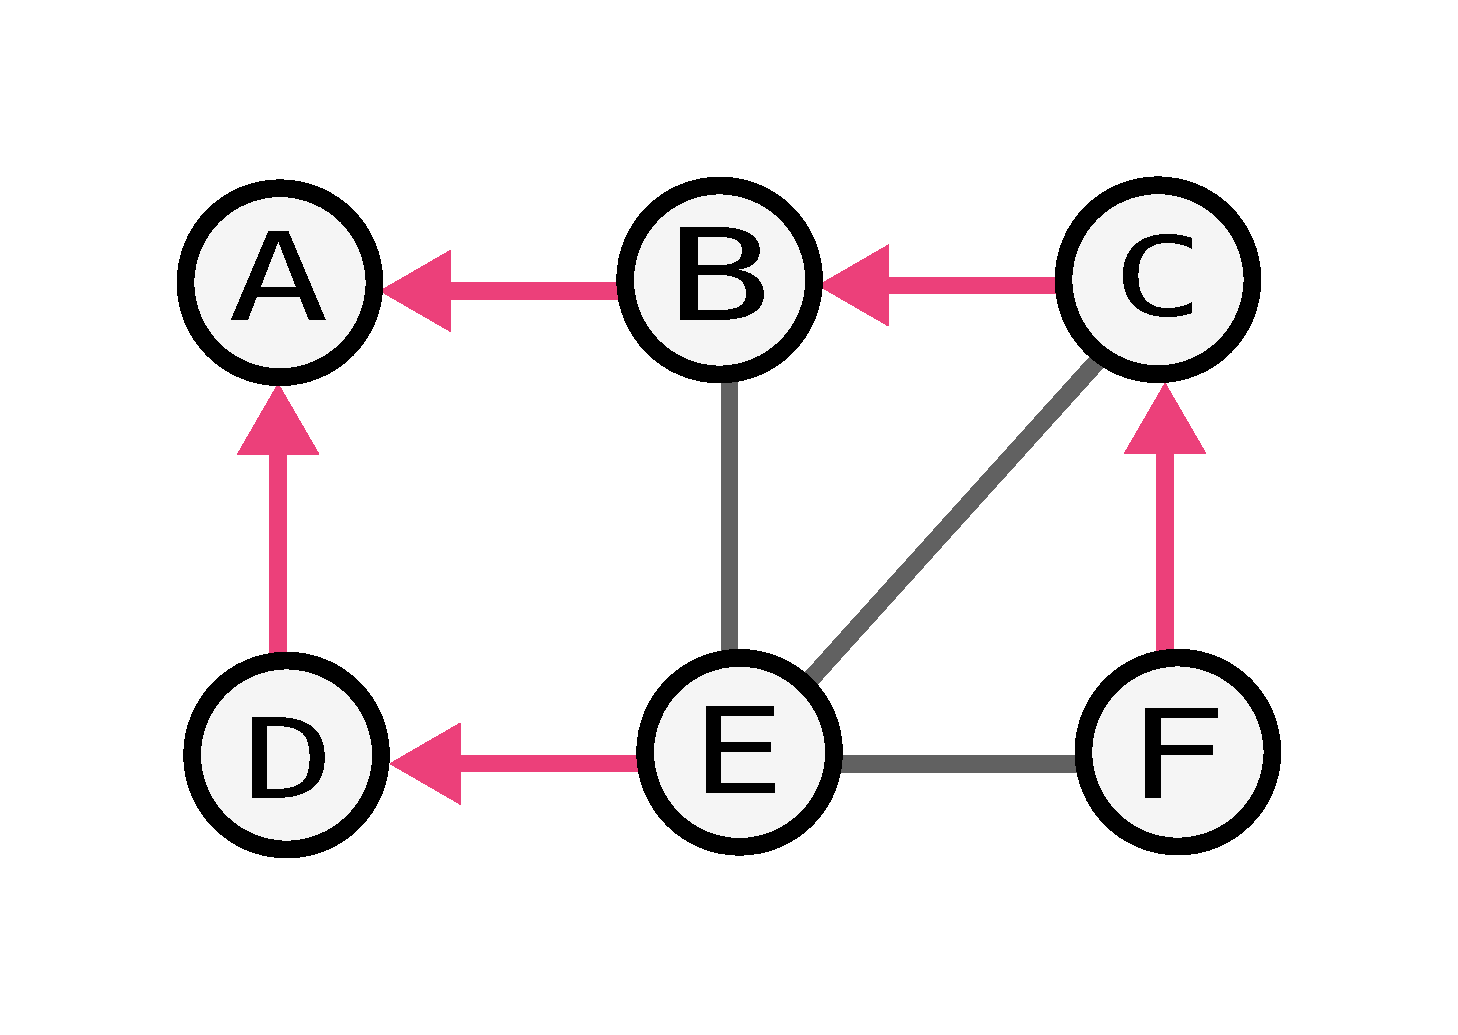
\includegraphics[width=0.5\paperwidth]{round3-end.pdf}
    \end{figure}
\end{frame}


\begin{frame}
    \frametitle{Why Synchrony?}
    \begin{figure}
    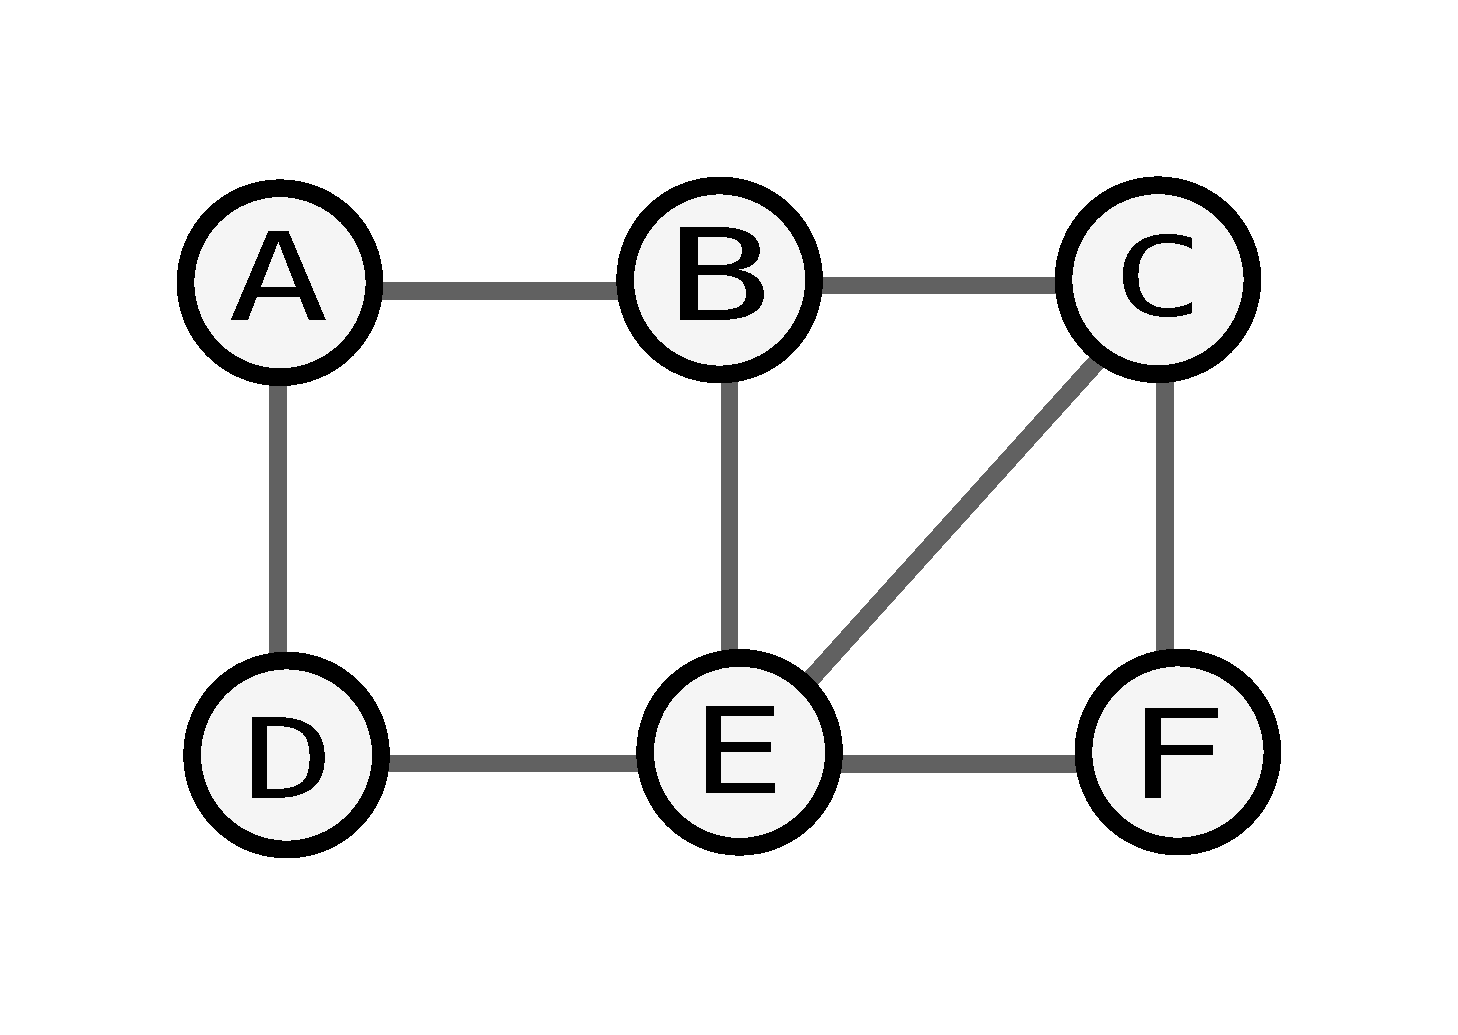
\includegraphics[width=0.5\paperwidth]{base.pdf}
    \end{figure}
\end{frame}

\begin{frame}
    \frametitle{Why Synchrony?}
    \begin{figure}
    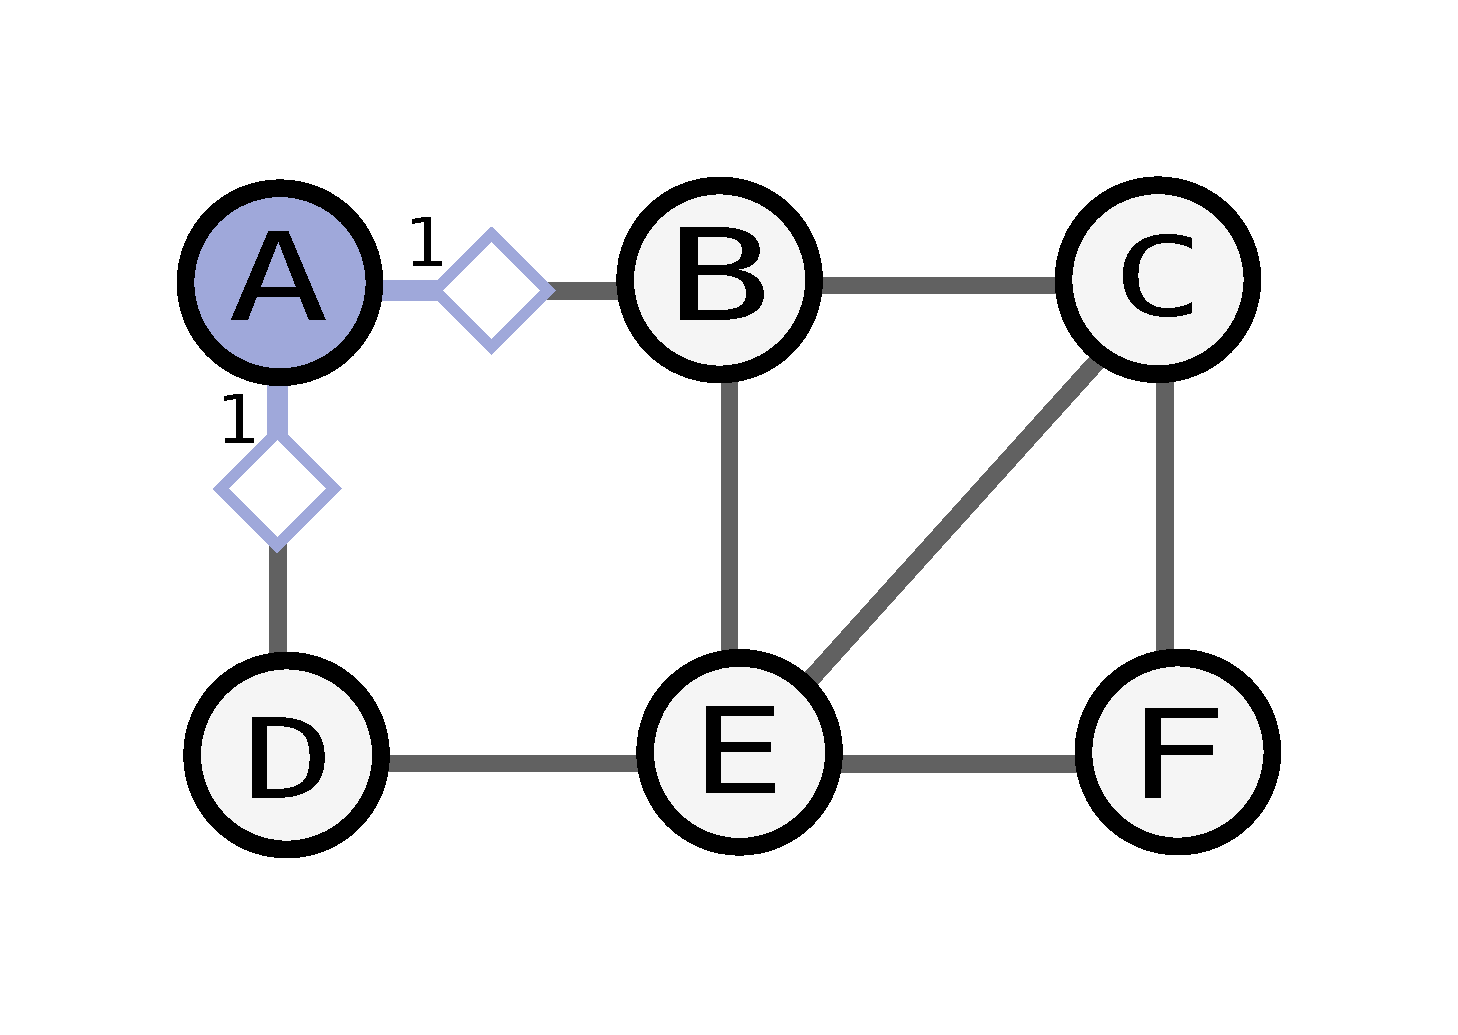
\includegraphics[width=0.5\paperwidth]{round1.pdf}
    \end{figure}
\end{frame}

\begin{frame}
    \frametitle{Why Synchrony?}
    \begin{figure}
    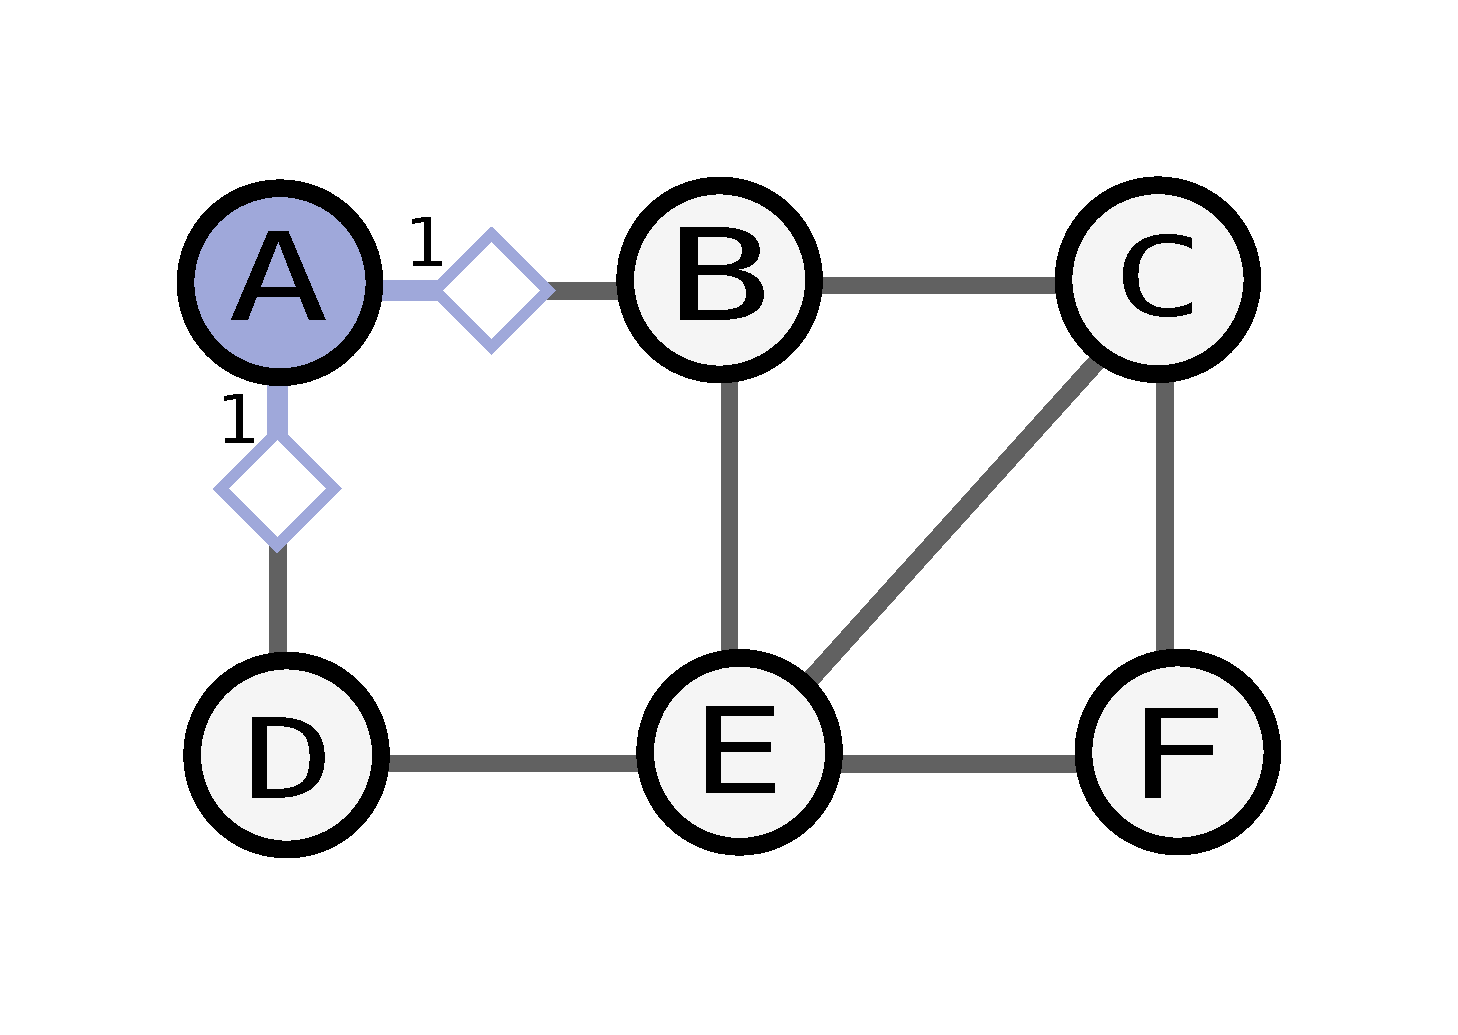
\includegraphics[width=0.5\paperwidth]{round1.pdf}
    \end{figure}
\end{frame}

\begin{frame}
    \frametitle{Why Synchrony?}
    \begin{figure}
    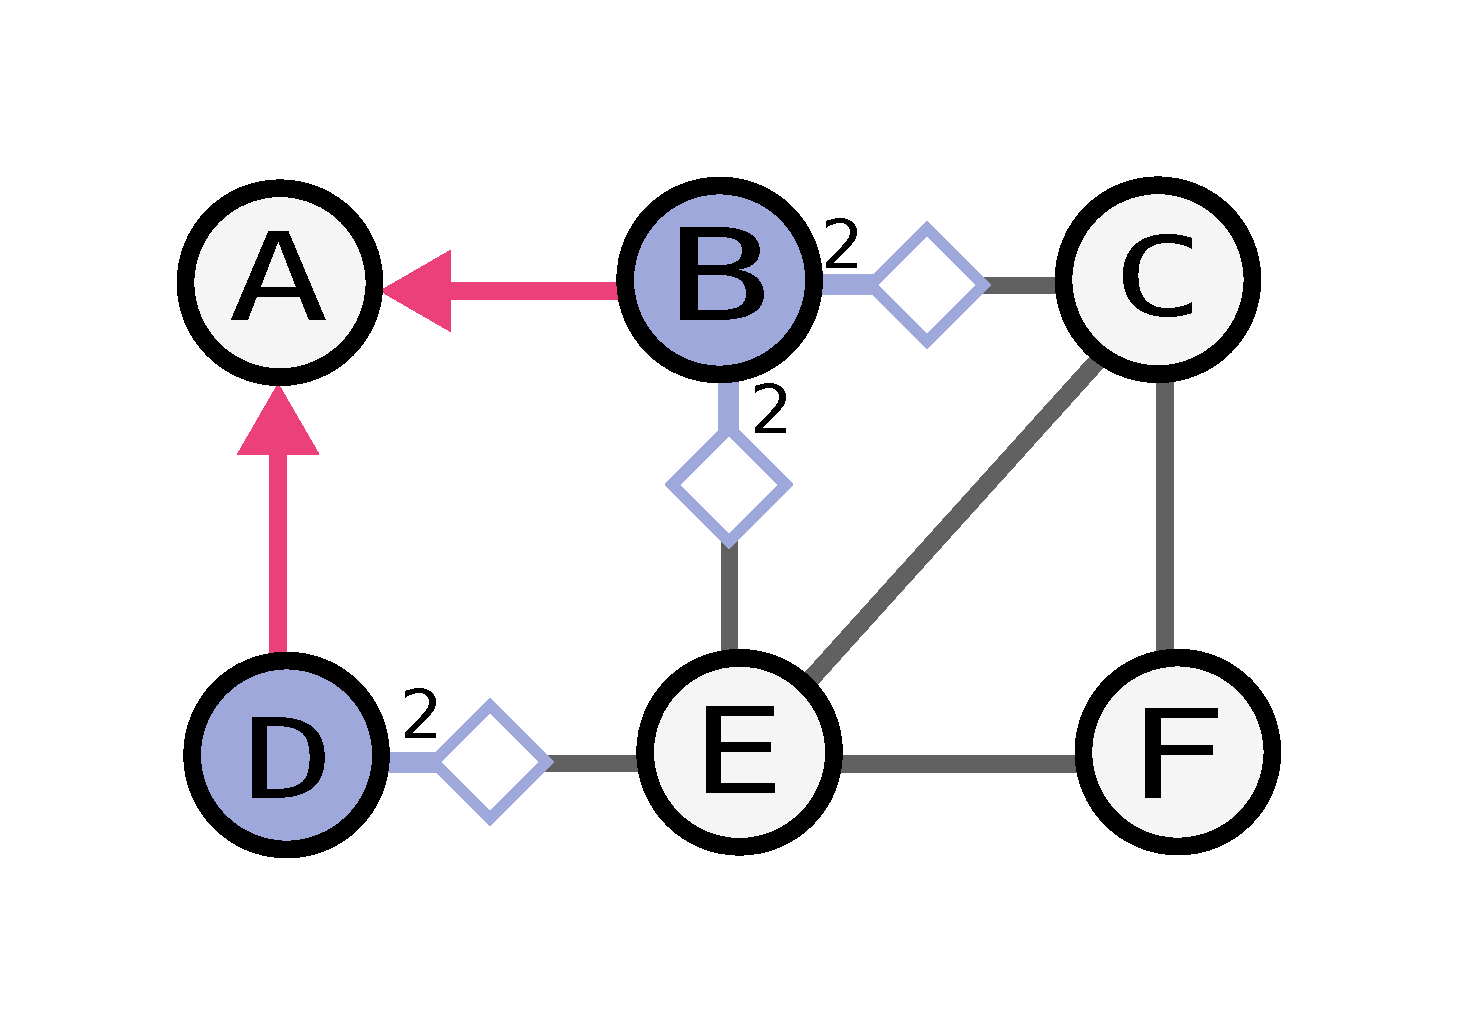
\includegraphics[width=0.5\paperwidth]{round2.pdf}
    \end{figure}
\end{frame}


\begin{frame}
    \frametitle{Why Synchrony?}
    \begin{figure}
    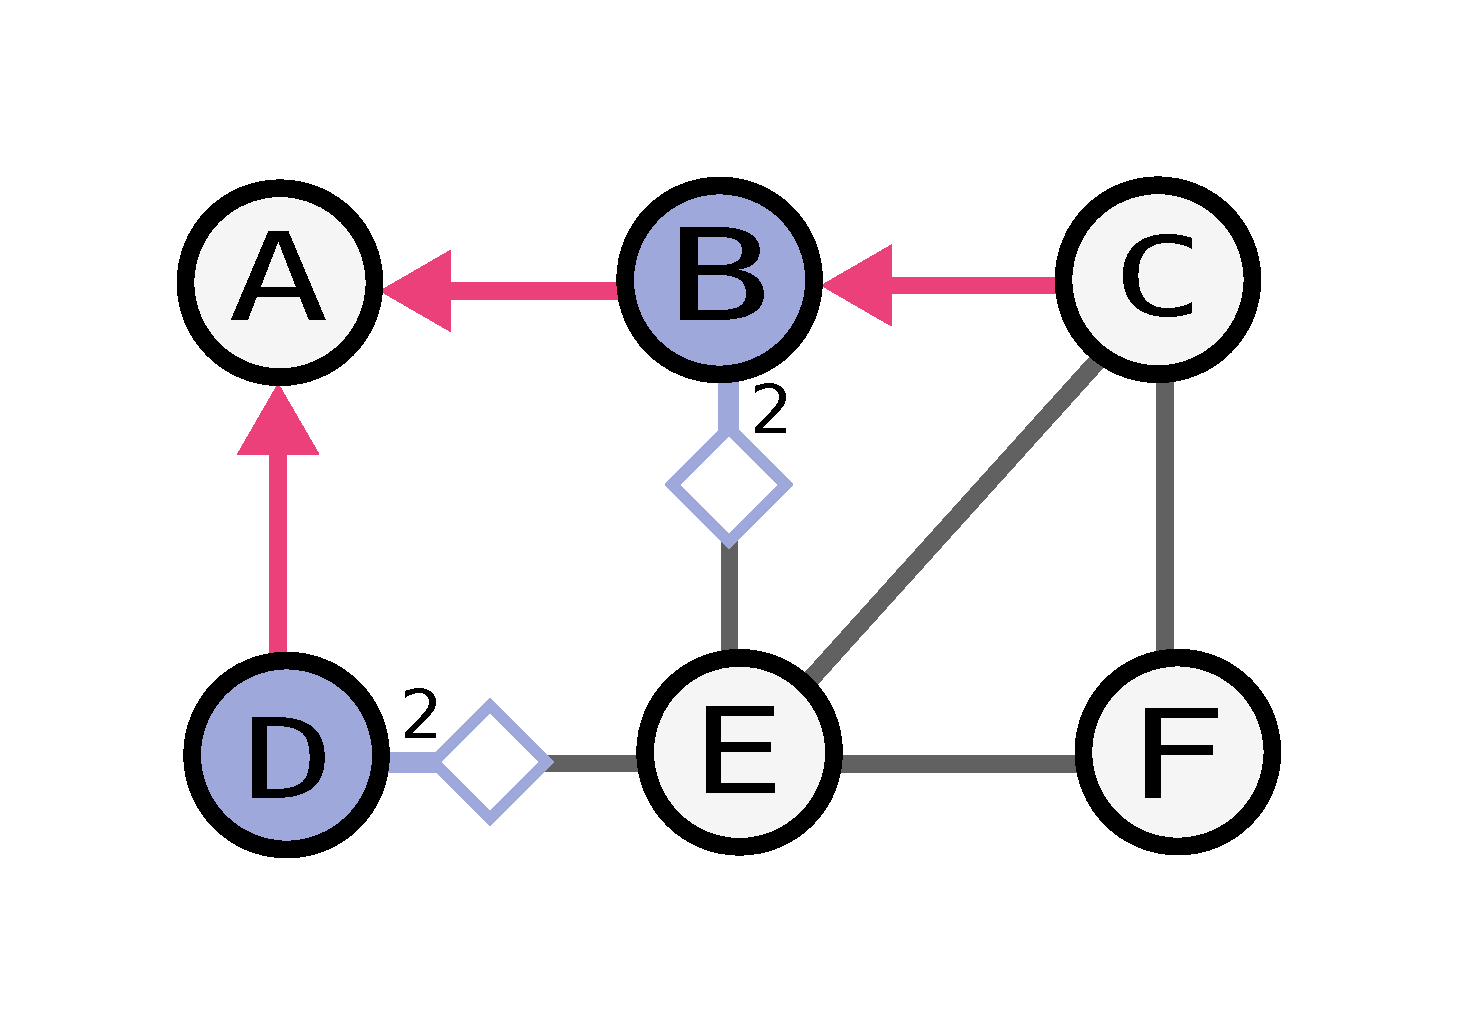
\includegraphics[width=0.5\paperwidth]{round2-fuckup-end.pdf}
    \end{figure}
\end{frame}

\begin{frame}
    \frametitle{Why Synchrony?}
    \begin{figure}
    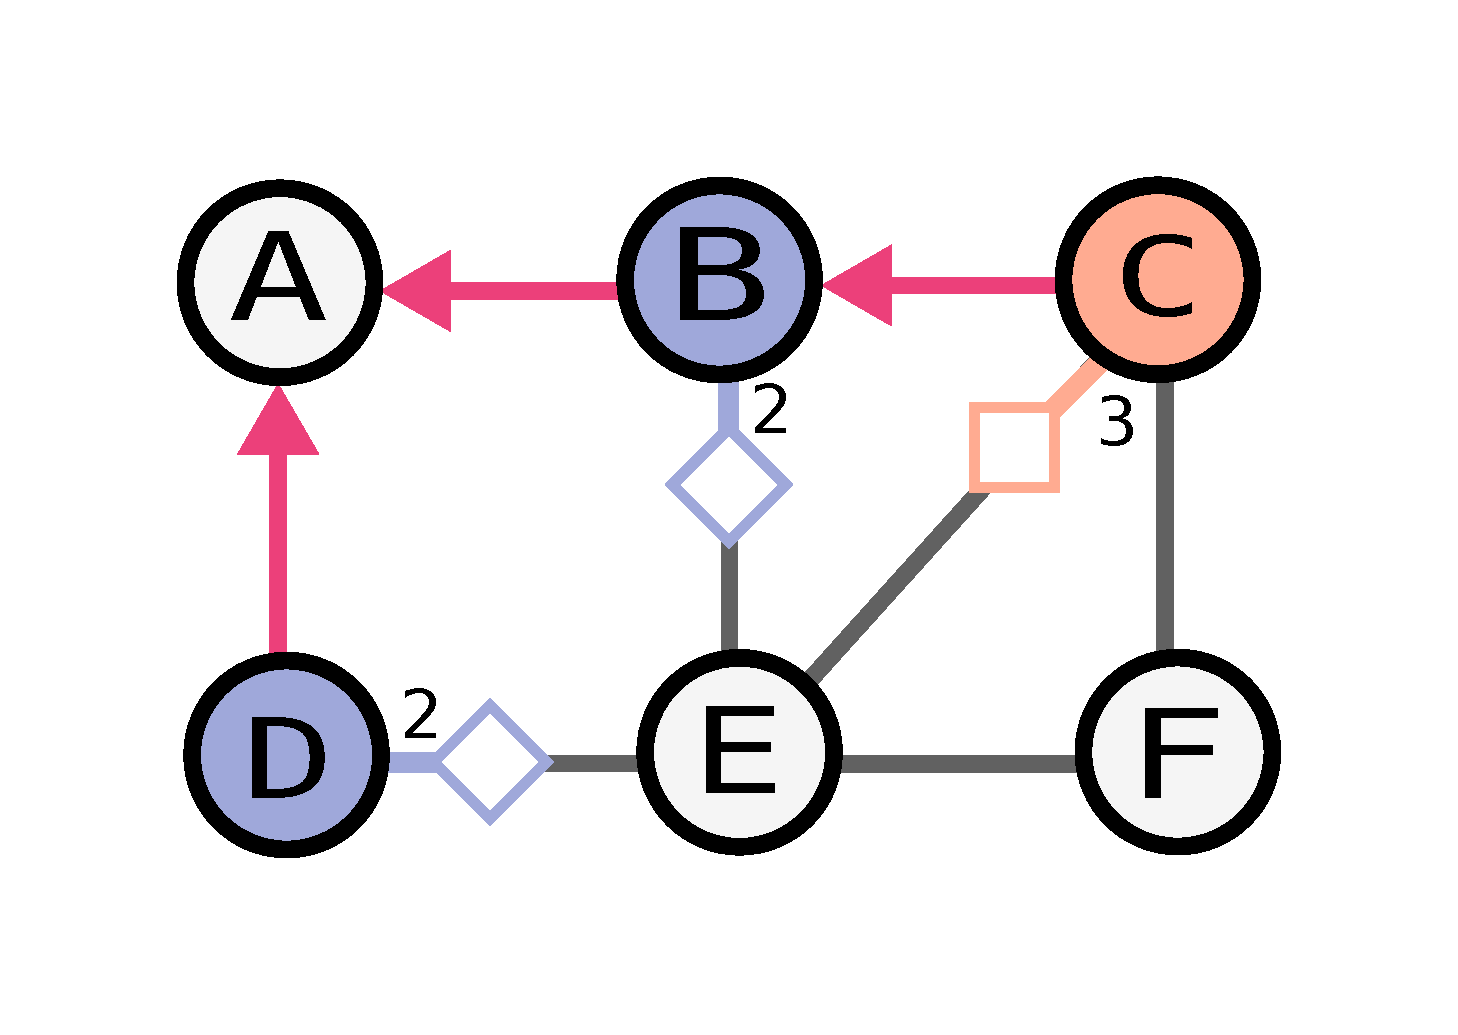
\includegraphics[width=0.5\paperwidth]{round3-fuckup.pdf}
    \end{figure}
\end{frame}


\begin{frame}
    \frametitle{Why Synchrony?}
    \begin{figure}
    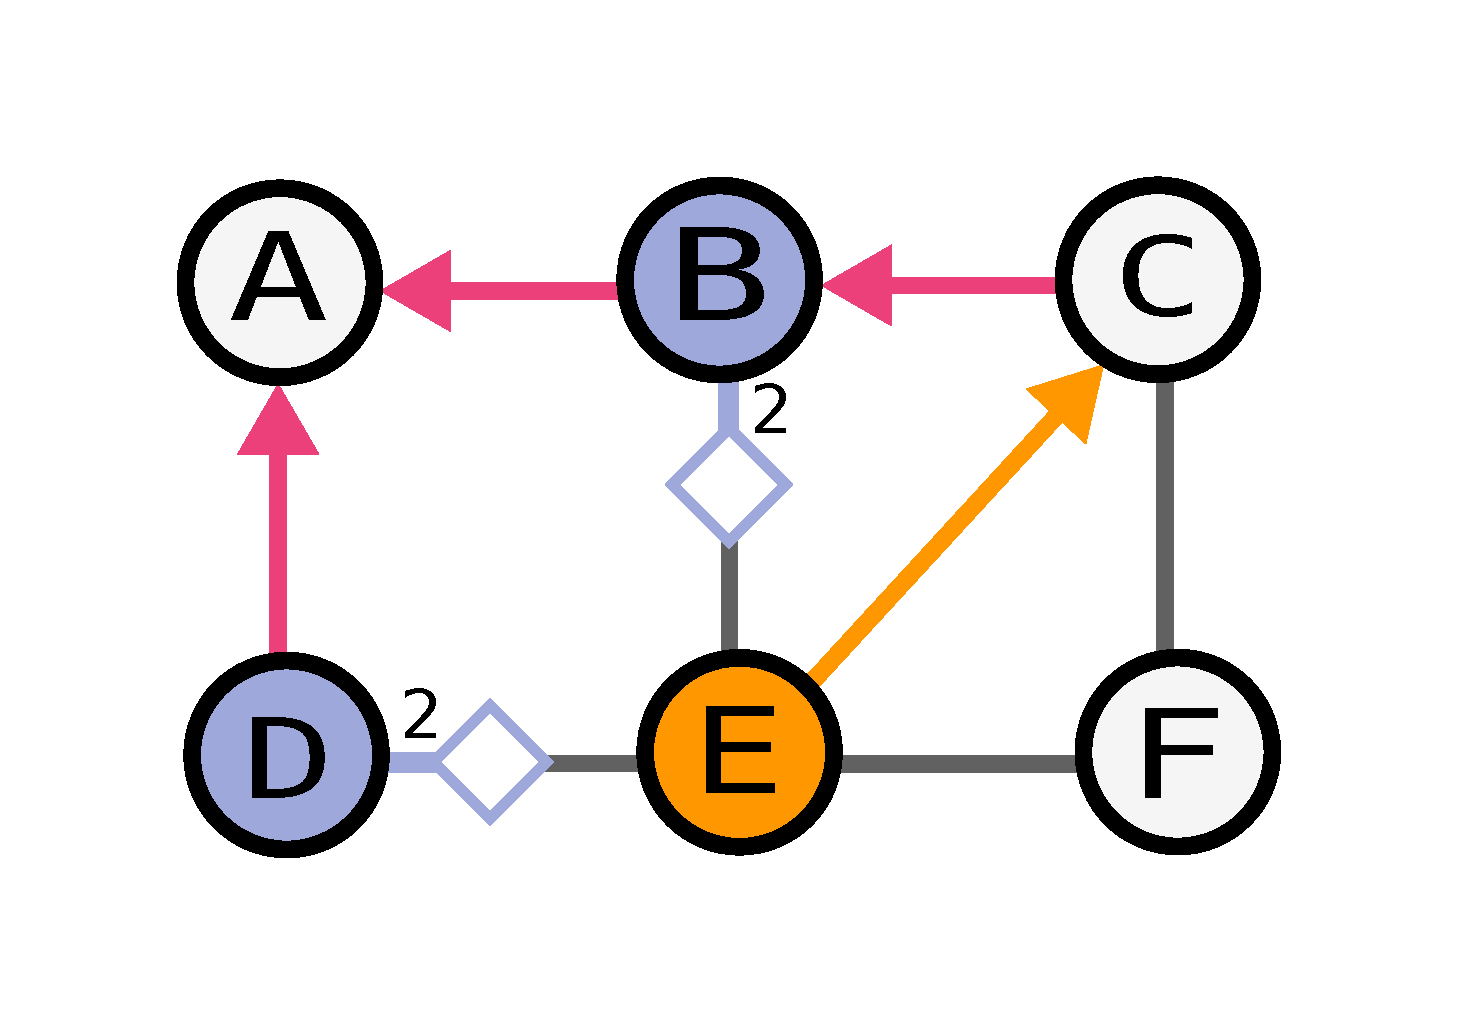
\includegraphics[width=0.5\paperwidth]{round3-fuckup-end.pdf}
    \end{figure}
\end{frame}

\begin{frame}[fragile]
    \frametitle{Synchronous BFS (Pseudocode)}
    \begin{itemize}
        \item Assume root begins computation.
        \item Algorithm is synchronous.
    \end{itemize}
    \pause

    \begin{minted}{python}
    def bfs_spanning_tree(self):
    \end{minted}
    \pause
    \begin{minted}{python}
      if self.id == ROOT_ID:
        self.visited = True; self.depth = 0;
        for n in self.neighbours: n.send(self.id)
    \end{minted}
    \pause
    \begin{minted}{python}
      for round in range(1, DIAMETER+1):
        if not self.visited: # if visited, skip
    \end{minted}
    \pause
    \begin{minted}{python}
          if self.queries: # if we have a query
            # randomly choose from queries
            parent = random.choice(self.query)
            self.visited = True
            self.depth = round
    \end{minted}
    \pause
    \begin{minted}{python}
            # synchronous
            for n in self.neighbours: n.send(self.id)
        self.queries = [];
    \end{minted}
\end{frame}

\begin{frame}[fragile]
    \frametitle{Synchronous BFS (Ending earlier if visited)}

    \begin{minted}{text}
    def bfs_spanning_tree(self):
    \end{minted}
    \begin{minted}{text}
      if self.id == ROOT_ID:
        self.depth = 0;
        for n in self.neighbours: n.send(self.id)
    \end{minted}
    \begin{minted}{python}
        return # early-exit for root node
    \end{minted}
    \begin{minted}{text}
      for round in range(1, DIAMETER+1):
    \end{minted}
    \begin{minted}{text}
          if self.queries: # if we have a query
            # randomly choose from queries
            parent = random.choice(self.query)
            self.visited = True
            self.depth = round
    \end{minted}
    \begin{minted}{text}
            # synchronous
            for n in self.neighbours: n.send(self.id)
    \end{minted}
    \begin{minted}{python}
            return # early-exit for child
    \end{minted}
\end{frame}

\begin{frame}[fragile]
    \frametitle{Synchronous BFS (Learning children)}
    \begin{itemize}
        \item Assume root begins computation.
        \item Algorithm is synchronous.
    \end{itemize}

    \begin{minted}{text}
    def bfs_spanning_tree(self):
    \end{minted}
    \begin{minted}{text}
      if self.id == ROOT_ID:
        self.visited = True; self.depth = 0;
        for n in self.neighbours: n.send(self.id)
    \end{minted}
    \begin{minted}{text}
      for round in range(1, DIAMETER+1):
    \end{minted}
    \begin{minted}{python}
        if self.visited: # if visited, wait for children
          for q in self.queries: self.children.append(q)
    \end{minted}
    \begin{minted}{text}
        else: # if not visited, run code
          if self.queries: # if we have a query
            # randomly choose from queries
            parent = random.choice(self.query)
            self.visited = True
            self.depth = round
    \end{minted}
    \begin{minted}{text}
            # synchronous
            for n in self.neighbours: n.send(self.id)
    \end{minted}
    \begin{minted}{python}
            parent.send(self.id) # send to parent
    \end{minted}
    \begin{minted}{text}
        self.queries = [];
    \end{minted}
\end{frame}

\begin{frame}
    \frametitle{Complexities}
    \pause
    \begin{itemize}
        \item Local space for $a$: $|\{ v : (a, v) \in E \}|$ (\#of incident edges) \pause
        \item $|Diameter|$ rounds. \pause
        \item 1 or 2 messages / edge. $\text{Message complexity} \leq 2|E|$.
    \end{itemize}
\end{frame}


\begin{frame}
    Thank you!
\end{frame}

\begin{frame}
    \frametitle{Asynchronous Bounded Delay Network}
    \begin{itemize}
    \item All processes have physical clocks: \textbf{need not be synchronized}.
    \item Message delivery time is bounded by constant $\mu \in \mathbb R$.
    \end{itemize}
    % Converting bounded delay to synchronous (Gerard Tel, Chapter 12)
\end{frame}

\begin{frame}
    \frametitle{ABD Synchronizers: Bounded Delay $\rightarrow$ Synchronized}
    \begin{itemize}
    \item All processes have physical clocks: \textbf{need not be synchronized}.
    \item Message delivery time is bounded by constant $\mu \in \mathbb R$.
    \end{itemize}

    \begin{block}{Key idea}
        Chunk "real time" into units of $\mu$. Each $\mu$ block of time
        behaves like a logical synchronized tick!
    \end{block}
    % Converting bounded delay to synchronous (Gerard Tel, Chapter 12)
\end{frame}

\begin{frame}
    \frametitle{Formal definition of synchronous processes $p$}
    \begin{itemize}
        \item $p \equiv (S, I, M\mathcal G, \vdash)$ \pause
        \item $S \equiv \text{set of states}$. \pause
        \item $I \subseteq S \equiv \text{set of initial states}$. \pause
        \item $M\mathcal G : S \rightarrow 2^M \equiv \text{message generating \textbf{function}}$. \pause
        \item $\vdash ~\subseteq S \times 2^M \subset S \equiv \text{transition \textbf{relation}}$. We write 
            $(s, M) \vdash s'$ for $(s, M, s') \in \vdash$.  \pause
        \item Process starts at state $s_0 \in I$.  
        \pause
        \item in state $s$, process sends a collection of messages $M\mathcal G(s)$.
        \pause
        \item \textbf{Before} next pulse, it receives \textit{all} messages $M$ sent to it in this pulse.
        \pause
        \item It then enters a state $s'$ such that $(s, M) \vdash s'$.
        \pause
        \item Note that $M\mathcal G$ is \textbf{deterministic}.
                All the nondeterminism is in the relation $(s, M) \vdash s'$.
    \end{itemize}
\end{frame}

\begin{frame}
    \frametitle{Formal definition of synchronous system $\mathbb P$}
    \begin{itemize}
        \item $\mathbb P \equiv (p_1, p_2, \dots, p_n)$ where each $p_i \equiv (S_i, I_i, M\mathcal G_i, \vdash_i)$
            is a synchronous process, is a synchronous system. \pause
        \item Transition system $Tr \equiv (S, \mathcal I, \rightarrow)$. \pause
        \item $S \equiv \prod_i S_i$ is the state space of the transition system. \pause
        \item $\mathcal I \equiv \prod_i I_i$ is the set of initial states. \pause
        \item $\rightarrow \subseteq S \times S$ is the transition relation.
            \begin{align*}
            &(s_1, s_2, \dots s_n) \rightarrow (s_1', s_2', \dots, s_n')\\
            &\quad \text{iff} \quad\forall p_i \in \mathbb P; (s_i, \{ \text{messages to $p_i$ from $p_{-i}$} \}) \vdash s_i'
        \end{align*}
            
    \end{itemize}
\end{frame}

\begin{frame}
    % Spanning tree computation: async version
\end{frame}


\end{document}
